\documentclass[journal,hidelinks]{IEEEtran}
\usepackage[utf8]{inputenc}
\usepackage[
  pdftitle={Assignment \#1},
  pdfauthor={Andrei Purcarus},
  pdfsubject={ECSE-534 -- Analog Microelectronics}
]{hyperref}
\usepackage{graphicx}
\usepackage[all]{hypcap}
\usepackage{cleveref}
\usepackage{indentfirst}
\usepackage[per-mode=symbol]{siunitx}

\title{ECSE-534 \\ Analog Microelectronics \\ Assignment \#1}
\author{Andrei~Purcarus,~260631911,~\IEEEmembership{McGill~University}}

\begin{document}
\sloppy

\maketitle

\begin{abstract}

A CMOS amplifier was analyzed using Cadence and its performance was characterized using DC, small signal AC, and transient analysis. The amplifier was found to meet its specifications, with unity gain stability, a DC gain of $\SI{54}{\deci\bel}$, and a unity gain bandwidth of $\SI{425}{\mega\hertz}$. In addition, the amplifier was found to have a weak phase margin of $\SI{0.8}{\degree}$, suggesting an area of possible improvement.

\end{abstract}

\section{Introduction}

\IEEEPARstart{T}{his} report follows the analysis of a CMOS amplifier that has been designed for unity gain stability in a 0.13 micron process from IBM. The amplifier in question is shown in \Cref{fig:opamp}. Note that all NFET transistors have their body connected to $V_{SS}$ and all PFET transistors have their body connected to $V_{DD}$.

\section{Bias Resistance}

Before the analysis, we must first set the bias resistance $R_{bias}$ such that the drain current in $M_5$ is between $\SI{100}{\micro\ampere}$ and $\SI{150}{\micro\ampere}$. To this end, we sweep the resistance value and simulate the drain current in $M_5$. The results are shown in \Cref{fig:rsweep}. Using this graph, we choose a bias resistance $R_{bias} = \SI{100}{\kilo\ohm}$.

\begin{figure}[!htb]
  \centering
  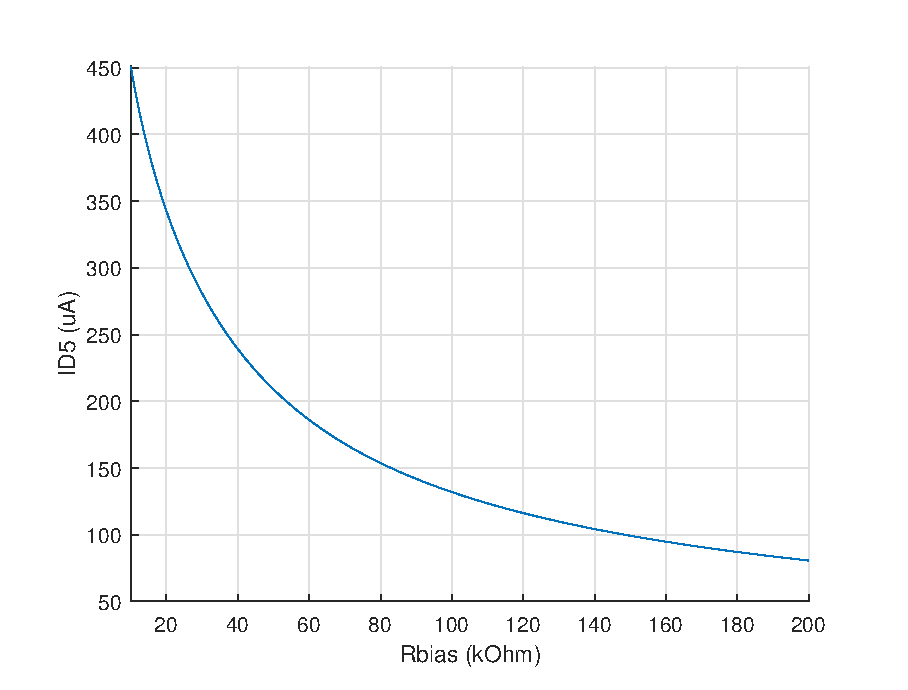
\includegraphics[width=\columnwidth]{rsweep.eps}
  \caption{Drain current in transistor $M_5$ as a function of $R_{bias}$.}
  \label{fig:rsweep}
\end{figure}

\section{DC Analysis}

Next, we measure the DC properties of the amplifier using the setup shown in \Cref{fig:dc_setup}, where the $\SI{1.2}{\volt}$ power supply has been omitted for clarity.

\begin{figure}[!htb]
  \centering
  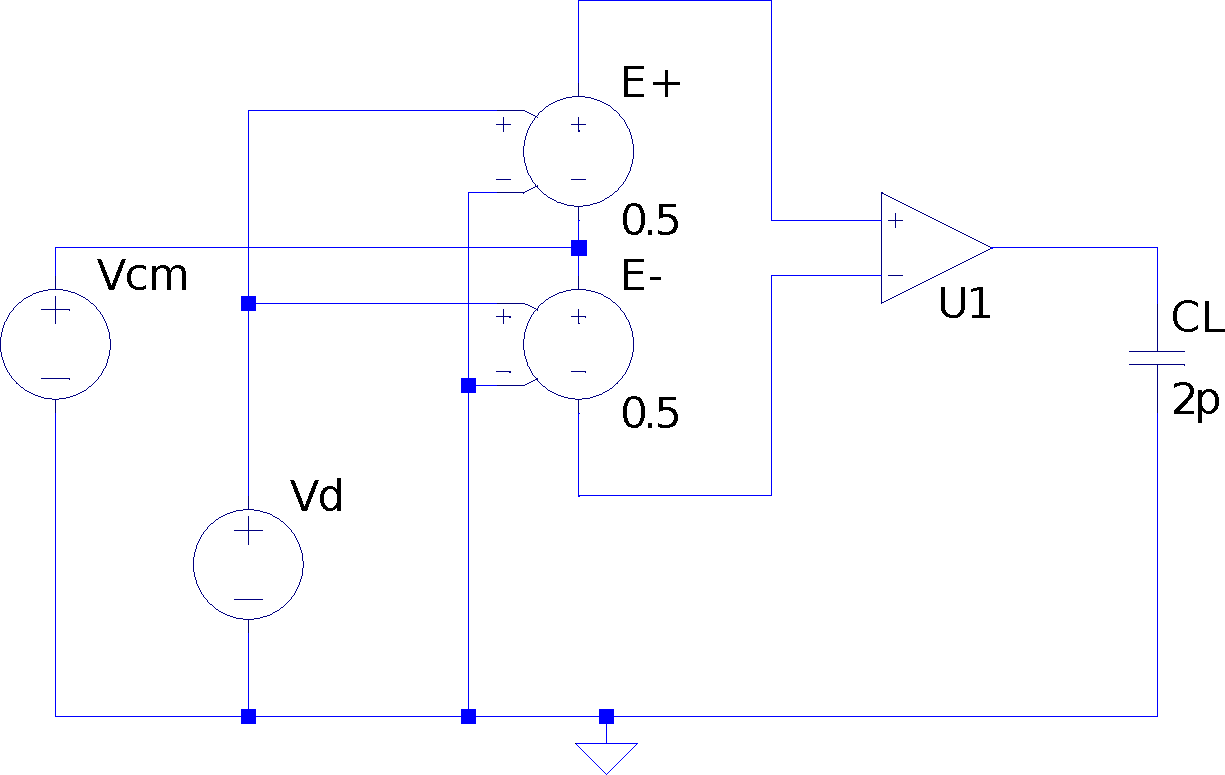
\includegraphics[width=\columnwidth]{dc_setup.pdf}
  \caption{A schematic of the setup used for measuring the DC and common mode properties of the amplifier.}
  \label{fig:dc_setup}
\end{figure}

We first sweep the common mode voltage $V_{cm}$ over the entire supply range and measure the output voltage, with $V_d = \SI{0}{\volt}$. The results are shown in \Cref{fig:dc_cm}. We see that the built-in voltage offset causes saturation regardless of common mode voltage.

\begin{figure}[!htb]
  \centering
  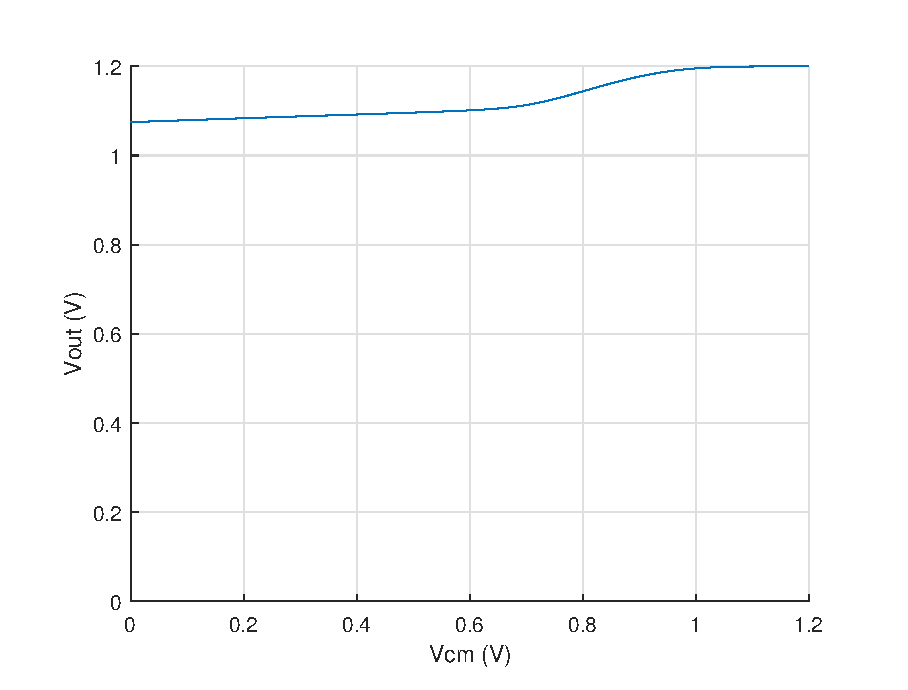
\includegraphics[width=\columnwidth]{dc_cm.eps}
  \caption{DC common mode transfer characteristic of the operational amplifier.}
  \label{fig:dc_cm}
\end{figure}

Then, we sweep the differential voltage $V_d$ from $\SI{-10}{\milli\volt}$ to $\SI{10}{\milli\volt}$, with $V_{cm} = \SI{0.6}{\volt}$ for proper biasing. The results are shown in \Cref{fig:dc_dm}. From this figure, we find that $V_{os} = \SI{-1.4}{\milli\volt}$.

\begin{figure}[!htb]
  \centering
  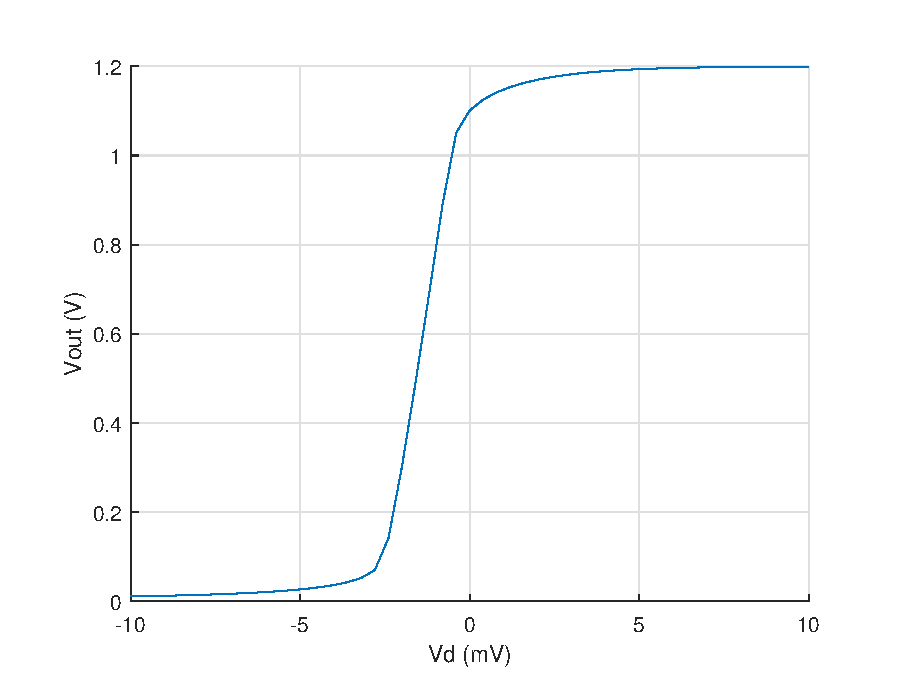
\includegraphics[width=\columnwidth]{dc_dm.eps}
  \caption{DC differential transfer characteristic of the operational amplifier.}
  \label{fig:dc_dm}
\end{figure}

To find the input and output voltage ranges, we plot the incremental voltage gain in \Cref{fig:dc_dm_gain}. We then choose the voltage range as being the range in which the incremental gain is at most $\SI{3}{\deci\bel}$ down from the peak value. Thus, we get an input voltage range of $\SI{-2.3}{\milli\volt}$ to $\SI{-0.5}{\milli\volt}$ and an output voltage range of $\SI{0.18}{\volt}$ to $\SI{1.0}{\volt}$.

\begin{figure}[!htb]
  \centering
  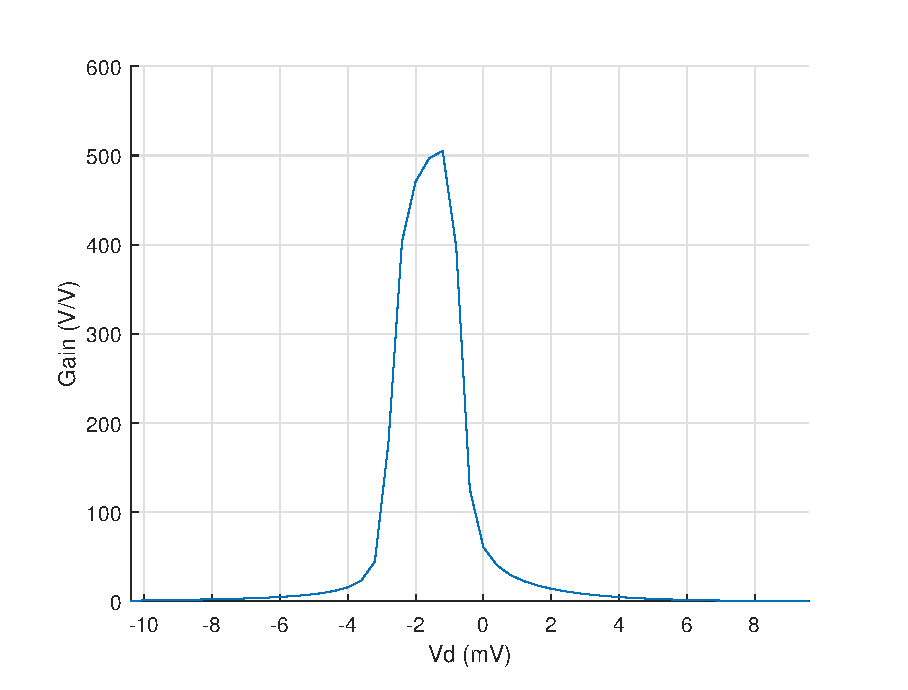
\includegraphics[width=\columnwidth]{dc_dm_gain.eps}
  \caption{DC incremental differential gain of the operational amplifier.}
  \label{fig:dc_dm_gain}
\end{figure}

\section{AC Analysis}

Next, we measure the AC properties of the amplifier. First, we measure the common mode frequency response using the setup in \Cref{fig:dc_setup}, keeping the DC component of $V_{cm} = \SI{0.6}{\volt}$ and setting $V_d = \SI{0}{\volt}$. The results are shown in \Cref{fig:ac_cm}. From this figure, we can see that the gain at low frequencies is $\SI{-24}{\deci\bel}$.

\begin{figure}[!htb]
  \centering
  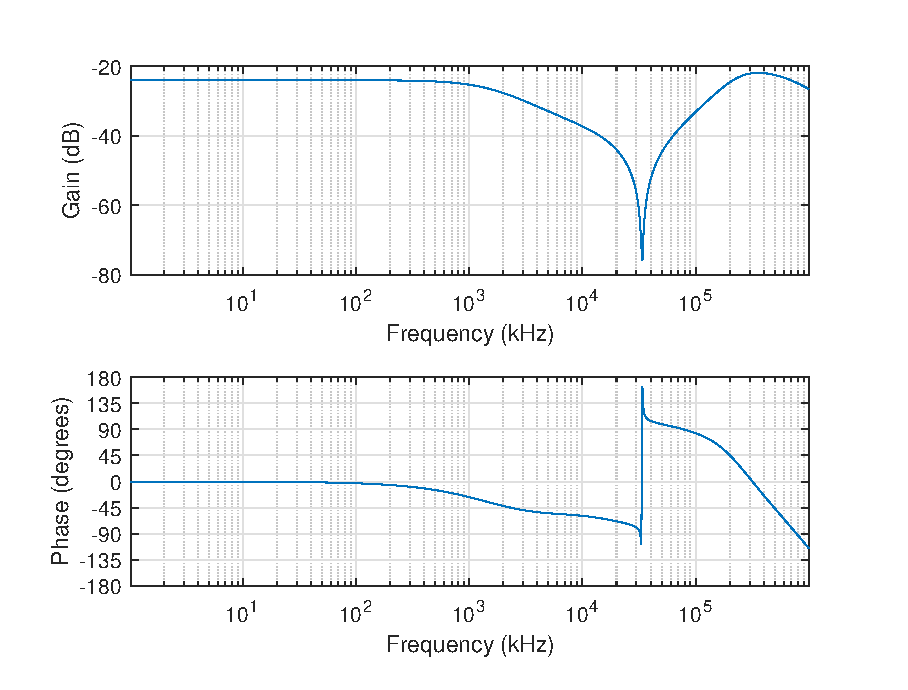
\includegraphics[width=\columnwidth]{ac_cm.eps}
  \caption{AC common mode frequency response of the operational amplifier.}
  \label{fig:ac_cm}
\end{figure}

Then, we measure the differential mode frequency response using the setup in \Cref{fig:ac_setup}, where the $\SI{1.2}{\volt}$ power supply has been omitted for clarity. In this setup, we have connected the output to the negative input at DC with a large inductor, ensuring bias stability. We then inject the signal through a large capacitor. These components are chosen so large that they do not affect the results of the AC analysis. $V_{bias}$ is set to $\SI{0.6}{\volt}$ for proper biasing.

\begin{figure}[!htb]
  \centering
  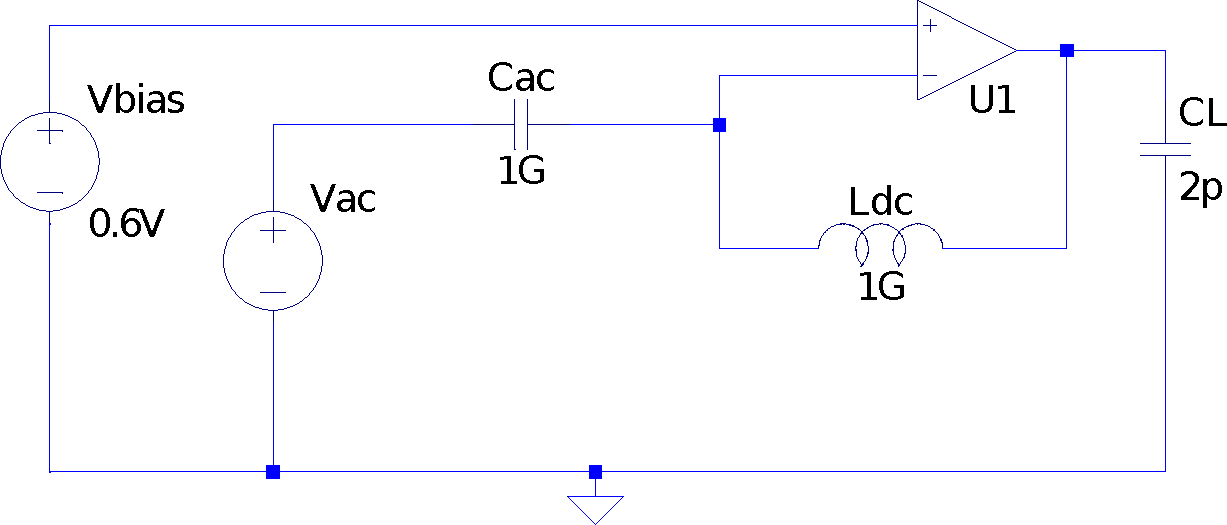
\includegraphics[width=\columnwidth]{ac_setup.pdf}
  \caption{A schematic of the setup used for measuring the AC properties of the amplifier.}
  \label{fig:ac_setup}
\end{figure}

The results of this analysis are shown in \Cref{fig:ac_dm}. From this graph, we can see that the low frequency gain is $\SI{54}{\deci\bel}$, the unity gain bandwidth is $\SI{425}{\mega\hertz}$, and the phase margin is $\SI{0.8}{\degree}$. We can also see that the amplifier has a pole at $\SI{320}{\kilo\hertz}$, a zero at around $\SI{100}{\mega\hertz}$, and two poles around $\SI{425}{\mega\hertz}$.

\begin{figure}[!htb]
  \centering
  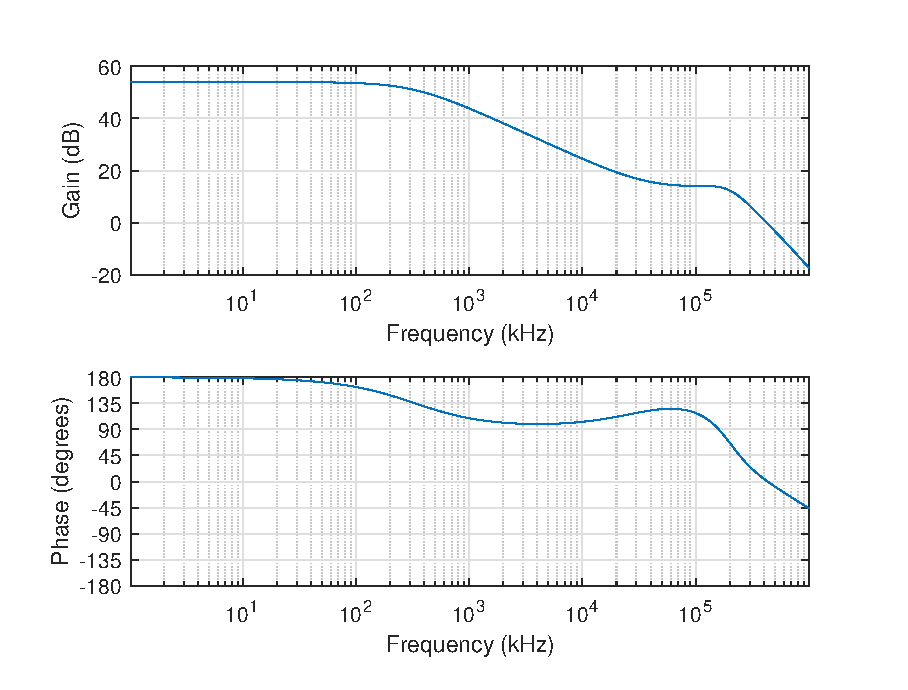
\includegraphics[width=\columnwidth]{ac_dm.eps}
  \caption{AC differential frequency response of the operational amplifier.}
  \label{fig:ac_dm}
\end{figure}

Next, we measure the AC noise of the amplifier using the same setup. Using $V_{ac}$ as our noise source, we get the output referred spectral noise density shown in \Cref{fig:ac_noise}. The noise was measured from $\SI{100}{\hertz}$ to $\SI{10}{\mega\hertz}$, with the RMS value calculated to be $\SI{6.3}{\milli\volt}$ over this bandwidth. We note that the noise is dominated by flicker noise.

\begin{figure}[!htb]
  \centering
  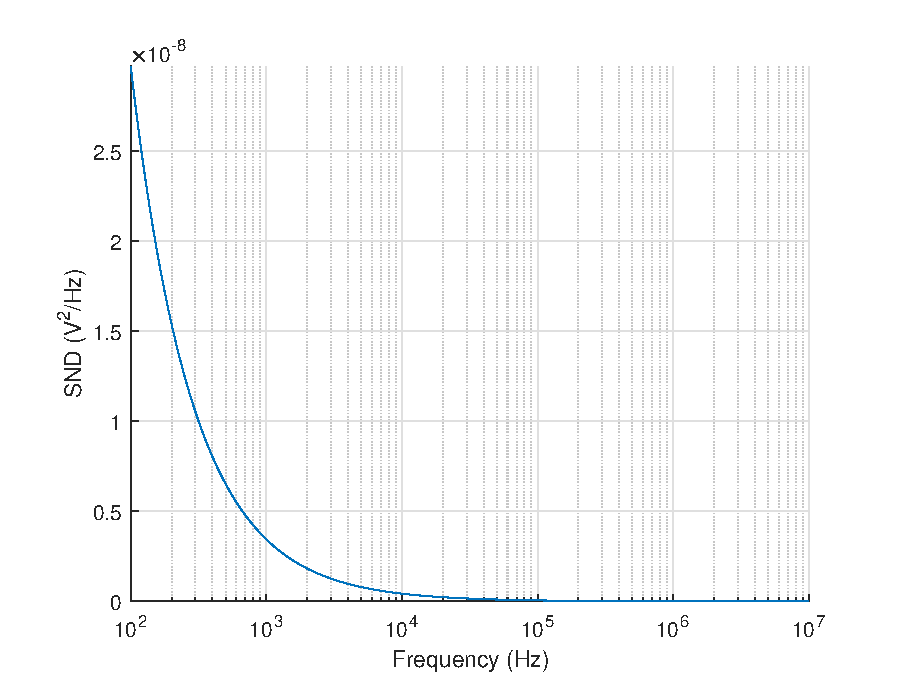
\includegraphics[width=\columnwidth]{ac_noise.eps}
  \caption{Output referred AC noise of the operational amplifier.}
  \label{fig:ac_noise}
\end{figure}

\section{Transient Analysis}

Finally, we measure the closed loop transient behaviour of the amplifier using the setup shown in \Cref{fig:tran_setup}, where the $\SI{1.2}{\volt}$ power supply has been omitted for clarity.

\begin{figure}[!htb]
  \centering
  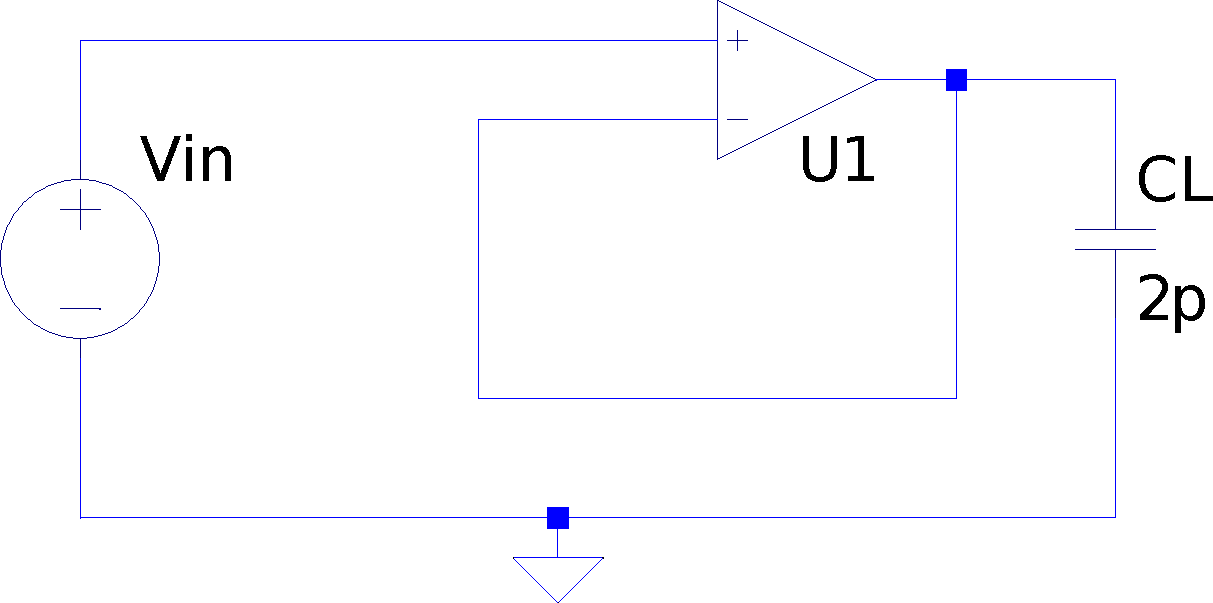
\includegraphics[width=\columnwidth]{tran_setup.pdf}
  \caption{A schematic of the setup used for measuring the closed loop transient properties of the amplifier.}
  \label{fig:tran_setup}
\end{figure}

First, we input a fast $\SI{100}{\milli\volt}$ pulse to the circuit, centered around a DC bias point of $\SI{0.6}{\volt}$. The resulting output is shown in \Cref{fig:tran_step}. From this graph, we can measure the slew rate as $\SI{64}{\volt\per\micro\second}$, the $\SI{10}{\percent}$ to $\SI{90}{\percent}$ rise time as $\SI{1.25}{\nano\second}$, and the $\SI{5}{\percent}$ settling time as $\SI{26}{\nano\second}$.

\begin{figure}[!htb]
  \centering
  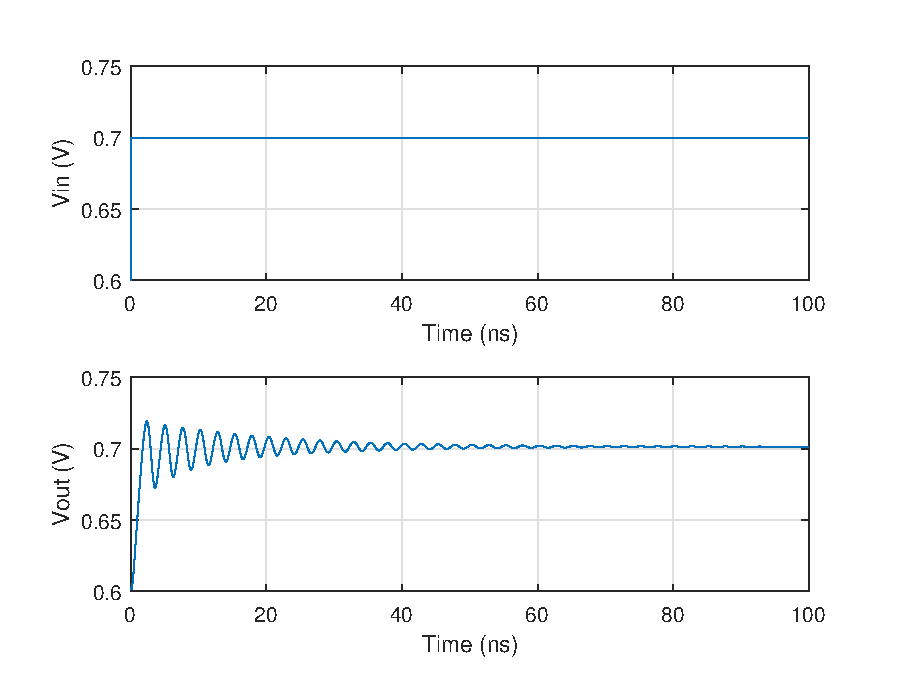
\includegraphics[width=\columnwidth]{tran_step.eps}
  \caption{Transient step response of the operational amplifier.}
  \label{fig:tran_step}
\end{figure}

Next, we measure clipping by using a large $\SI{1}{\kilo\hertz}$ sine wave as input to the circuit. The resulting output is shown in \Cref{fig:tran_clip}. From this, we find that the maximum input and output voltage ranges are both $\SI{0}{\volt}$ to $\SI{1.19}{\volt}$.

\begin{figure}[!htb]
  \centering
  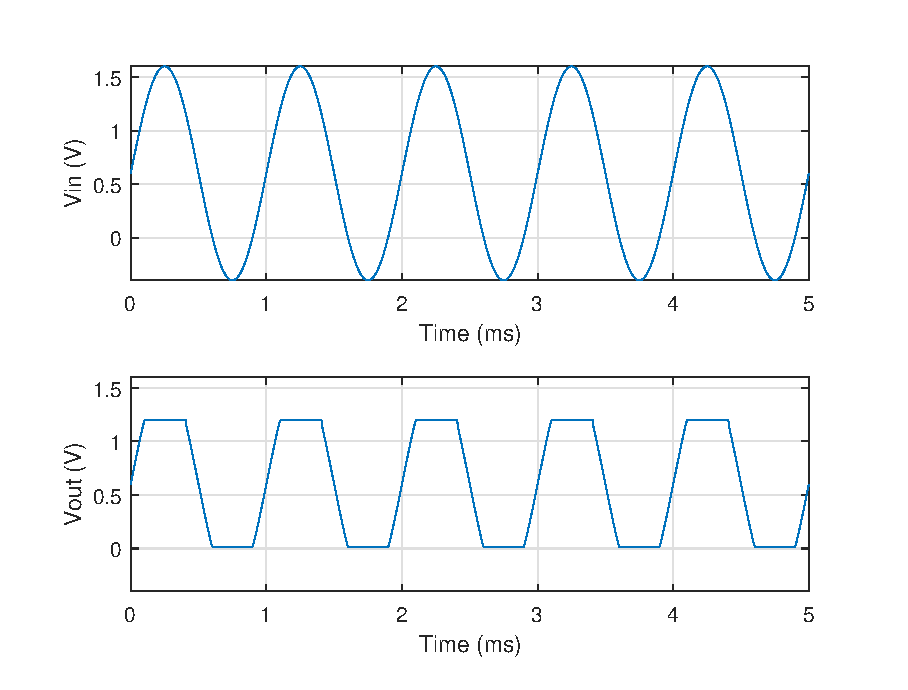
\includegraphics[width=\columnwidth]{tran_clip.eps}
  \caption{Transient response of the operational amplifier to a large $\SI{1}{\kilo\hertz}$ sine wave input.}
  \label{fig:tran_clip}
\end{figure}

Finally, we measure both common mode and differential mode distortion using the setup in \Cref{fig:dc_setup}. For this purpose, we add a DC offset equal to $V_{os}$ in series with $E_+$ to ensure adequate biasing. We first set the differential mode voltage $V_d = \SI{0}{\volt}$, and inject a common mode, $\SI{1}{\kilo\hertz}$, $\SI{100}{\milli\volt}$ amplitude sine wave on top of a $\SI{0.6}{\volt}$ DC offset. The resulting output is shown in \Cref{fig:tran_dist_cm}, and the total harmonic distortion was calculated to be $\SI{39.58}{\percent}$.

\begin{figure}[!htb]
  \centering
  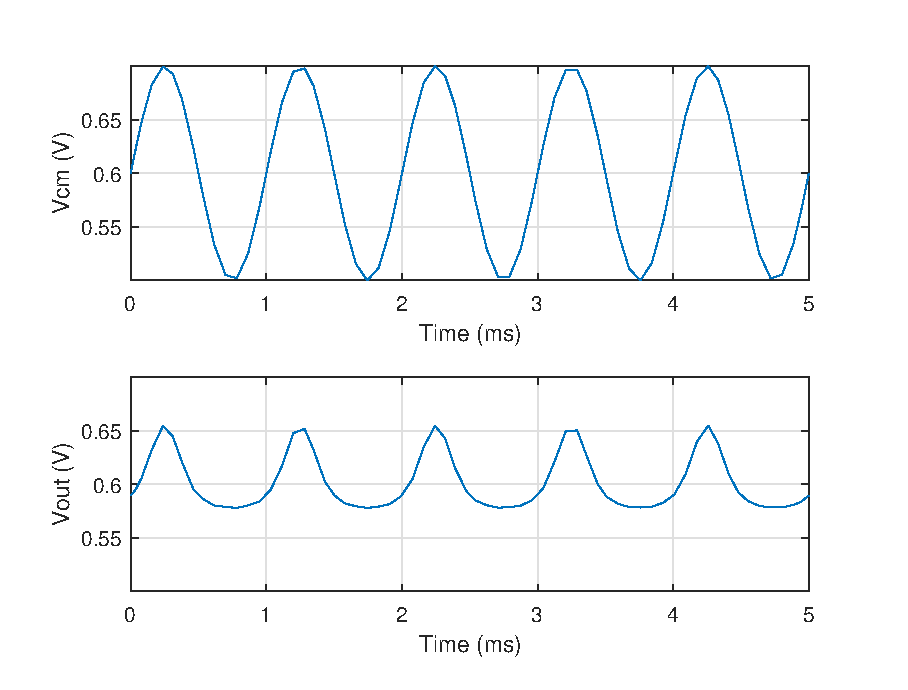
\includegraphics[width=\columnwidth]{tran_dist_cm.eps}
  \caption{Transient response of the operational amplifier to a $\SI{1}{\kilo\hertz}$, $\SI{100}{\milli\volt}$ amplitude common mode sine wave.}
  \label{fig:tran_dist_cm}
\end{figure}

Then, we fix the common mode voltage $V_{cm}$ at $\SI{0.6}{\volt}$, and set the differential voltage to a $\SI{1}{\kilo\hertz}$, $\SI{1.2}{\milli\volt}$ amplitude sine wave, which was chosen to get an output swing close to the limit. The resulting output is shown in \Cref{fig:tran_dist_dm}, and the total harmonic distortion was calculated to be $\SI{6.04}{\percent}$.

\begin{figure}[!htb]
  \centering
  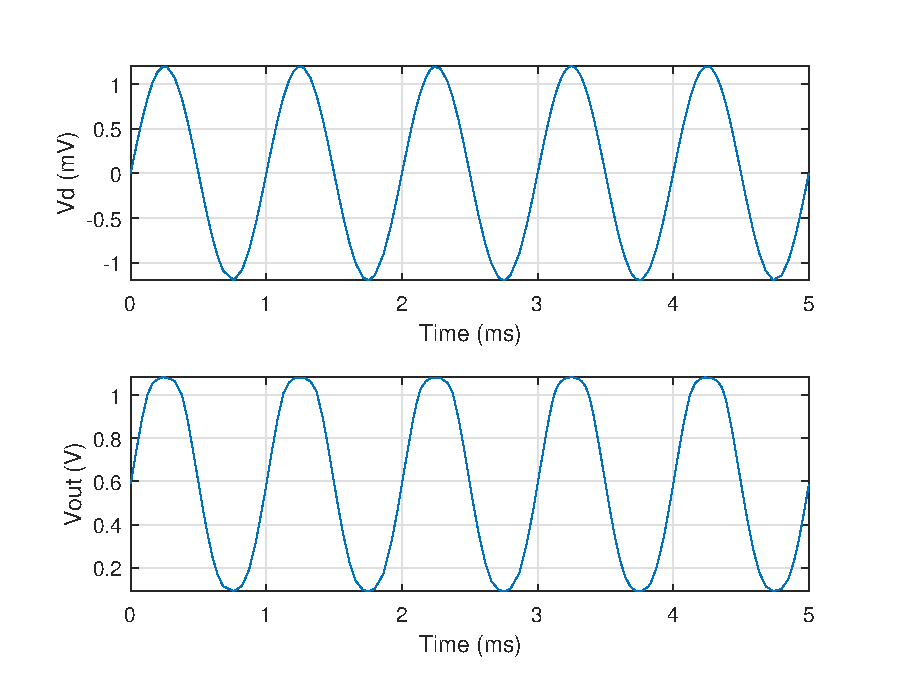
\includegraphics[width=\columnwidth]{tran_dist_dm.eps}
  \caption{Transient response of the operational amplifier to a $\SI{1}{\kilo\hertz}$, $\SI{1.2}{\milli\volt}$ amplitude differential sine wave.}
  \label{fig:tran_dist_dm}
\end{figure}

\begin{figure*}[!htb]
  \centering
  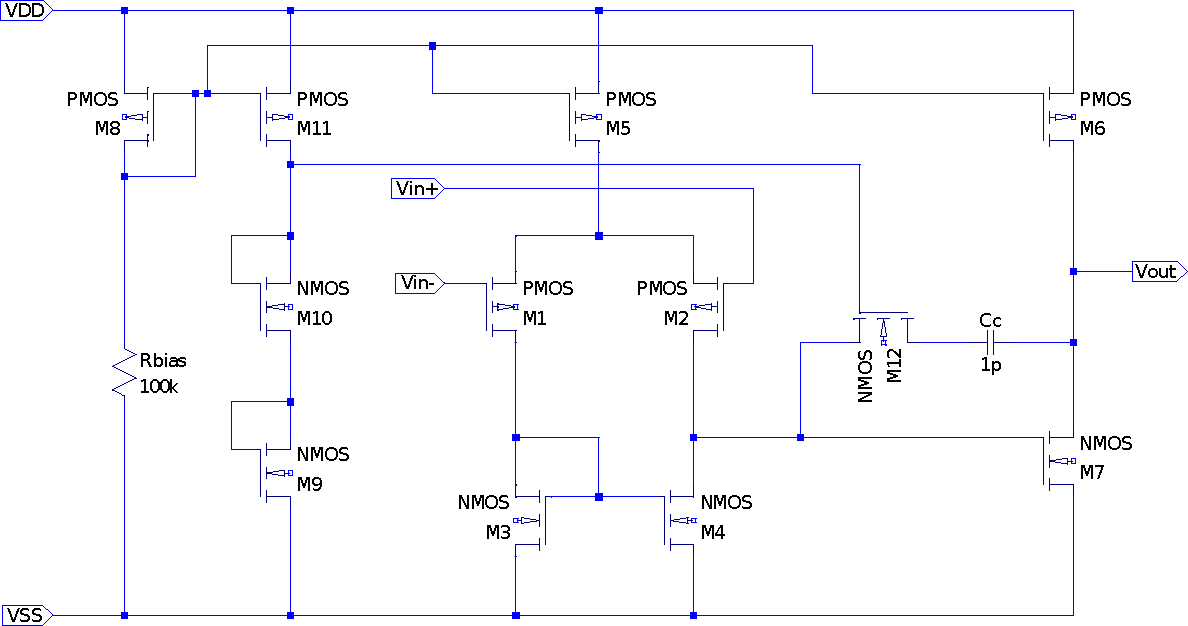
\includegraphics[width=\textwidth]{opamp.pdf}
  \caption{Schematic of the operational amplifier.}
  \label{fig:opamp}
\end{figure*}

\section{Conclusions}

In conclusion, the operational amplifier shown in \Cref{fig:opamp} was analyzed and its performance characterized using DC, small signal AC, and transient analysis. The amplifier performs its tasks adequately, with its main flaws being a low phase margin of $\SI{0.8}{\degree}$, and a relatively low gain of $\SI{54}{\deci\bel}$. However, it compensates for this with a high unity gain bandwidth of $\SI{425}{\mega\hertz}$.

\bibliographystyle{IEEEtran}
\bibliography{IEEEabrv,references}

\end{document}
